% -----------------------------------------------
% Template for ISMIR 2014
% (based on earlier ISMIR templates)
% -----------------------------------------------

\documentclass{article}
\usepackage{ismir2014,amsmath,cite}
\usepackage{graphicx}
\usepackage{brian}

% Title.
% ------
\title{Analyzing song structure with graph Laplacians}

% Single address
% To use with only one author or several with the same address
% ---------------
%\oneauthor
% {Names should be omitted for double-blind reviewing}
% {Affiliations should be omitted for double-blind reviewing}

% Two addresses
% --------------
%\twoauthors
%  {First author} {School \\ Department}
%  {Second author} {Company \\ Address}

% Three addresses
% --------------
\threeauthors
  {First author} {Affiliation1 \\ {\tt author1@ismir.edu}}
  {Second author} {\bf Retain these fake authors in\\\bf submission to preserve the formatting}
  {Third author} {Affiliation3 \\ {\tt author3@ismir.edu}}

% Four addresses
% --------------
%\fourauthors
%  {First author} {Affiliation1 \\ {\tt author1@ismir.edu}}
%  {Second author}{Affiliation2 \\ {\tt author2@ismir.edu}}
%  {Third author} {Affiliation3 \\ {\tt author3@ismir.edu}}
%  {Fourth author} {Affiliation4 \\ {\tt author4@ismir.edu}}

\begin{document}
%
\maketitle
%
\begin{abstract}
The abstract should be placed at the top left column and should contain about 150-200 words.
\end{abstract}
%
\section{Introduction}\label{sec:introduction}

\subsection{Our contributions}

\subsection{Related work}

\cite{serra2012unsupervised}

\cite{grohganz2013converting}

\subsection{Preliminaries}
% Define the graph laplacian, and the random-walk normalized variant
% define segmentation notation: 
%   d = input dimension
%   n = number of frames, 
%   s = number of segments, 
%   m = number of segment types
\section{Encoding repetition}
% Begin with nearest-neighbor linkage in some feature space
% Apply diagonal majority vote filtering
% Add the conveyor belt links
% Compute the graph laplacian, observe magic

Let $X = [x_1, x_2, \dots, x_n] \in \R^{d\times n}$ denote a $d$-dimensional time
series feature matrix, \eg, a chromagram or sequence of Mel-frequency cepstral 
coefficients).  As a first step toward detecting and representing repetition structure, 
we form a \emph{binary recurrence matrix} $R_k \in \{0,1\}^{n\times n}$, where $R_{ij}$ 
indicates that $x_i$ and $x_j$ are mutual $k$-nearest neighbors.
% FIXME: cite for recurrence matrix

If $X$ sufficiently captures the qualities of interest, and $k$ is large
enough, then repeated structures should appear as diagonal stripes in $R$.  





\subsection{The graph Laplacian}

\cite{chung1997spectral, von2007tutorial}


% Additional eigenvectors encode nested structures
% Pick a nice example here.  Maybe nirvana or green day?  Beatles would be fine too.

% Addenda:
% Fill in non-repeating regions with a planted clique
\begin{figure}
\centering
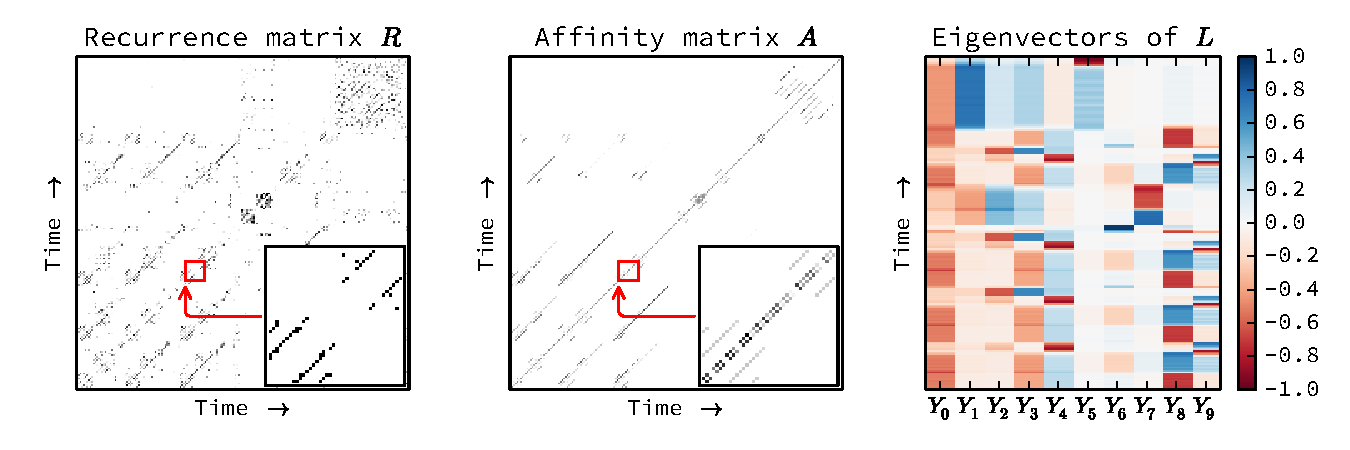
\includegraphics[width=\columnwidth]{figs/recurrence}
\caption{Upper-left: the raw recurrence matrix for \emph{The Beatles -- Come Together}; upper-right: the
recurrence matrix after diagonal filtering; lower-left: a close-up of the first 140 beats; lower-right the first
10 basis features, ordered bottom-to-top.  The first four rows encode the primary structural components.\label{recurrence}}
\end{figure}

 
\begin{figure*}
\centering
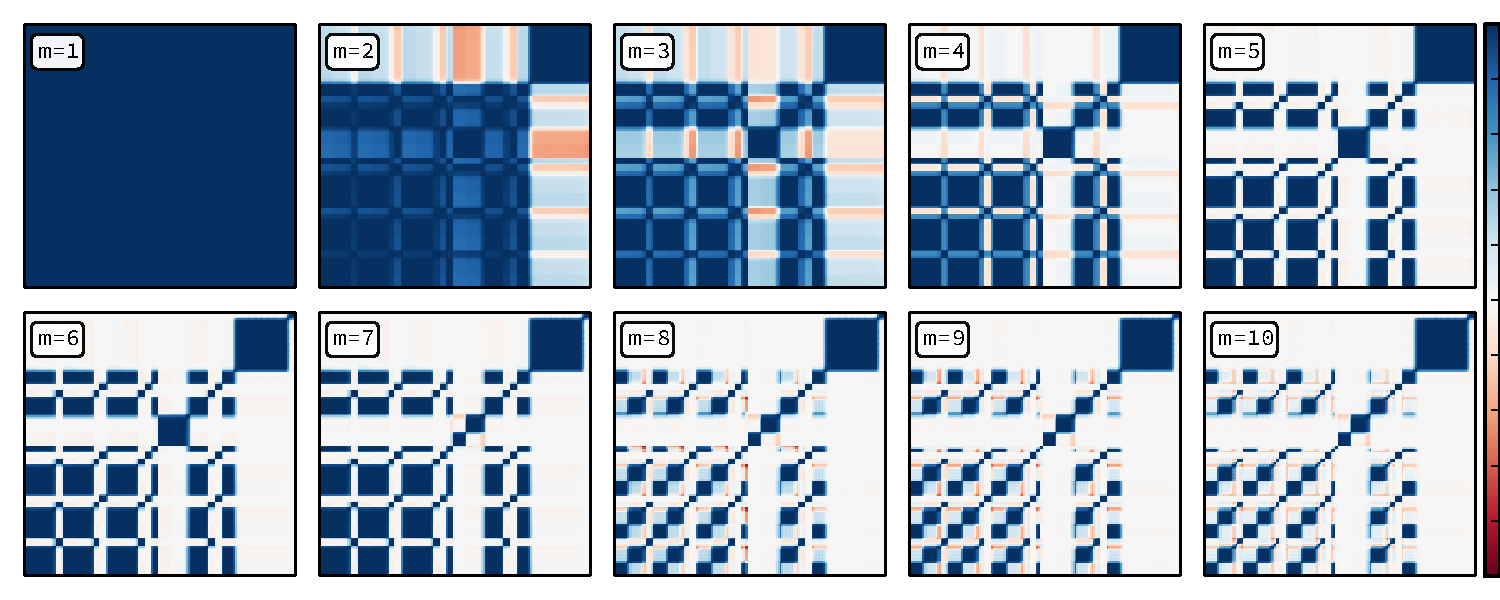
\includegraphics[width=\textwidth]{figs/lowrank}
\caption{Pairwise frame similarity using the first $5$ components for \emph{The Beatles -- Come Together}.  The first
(trivial) component ($m=1$) captures the entire song, and the second ($m=2$) separates the solo and outro from the
rest of the song.  Subsequent refinements separate the verses and refrains, and then encode internal structure.\label{lowrank}}
\end{figure*}

\section{Algorithms}

\subsection{Change-point detection}
% For a fixed number of segment types, how can we do change-point detection?
% Partition the sequential linkage graph A
% Use repetition features to define the edge weights
% Local bandwidth estimation, non-maximal suppresssion
% 1. Estimate the number of segments k
% 2. Score the partitioning by the spectral gap $\lambda_k$


\subsection{Structure annotation}
% For each m in 2 .. M:
%   boundaries[m], gap[m] = change_point(Y[:m])
% m <- argmax gap
% compute segment centroids over boundaries[m], and cluster by k-means with k=m
% return boundary times and segment labels

\section{Experiments}

\subsection{Data}

\subsection{Implementation}

\subsection{Results}

\section{Discussion}

\bibliography{refs}

\end{document}
